\chapter{Casos de prueba}
\section{Tabla de casos}
\begin{table}[H]
	\centering
	\captionof{figure}{Casos de prueba iniciales propuestos para el sistema}
	\begin{tabular}{l|c c c c|r r}
		\hline
		\multirow{2}*{\bf{ID}} & \multicolumn{4}{c|}{\textbf{Entradas}} & \multicolumn{2}{c}{\bf{Salidas}} \\
		\cline{2-7}
		& $BI_p$ & $BI_s$ & $R$ & $P_{H}$ & Obligatoriedad & Resultado \\
		\hline
		\hline
		CP1 & 0€ & 0€ & 0€ & 0€ & No & TBA \\
		CP2 & 8999€ & 0€ & 0€ & 0€ & No & TBA \\
		CP3 & 8999€ & 0€ & 0€ & 0€ & Sí & TBA \\
		CP4 & 9000€ & 0€ & 0€ & 0€ & Sí & TBA \\
		CP5 & 12449€ & 0€ & $I-1$€ & 0€ & Sí & TBA \\
		CP6 & 12450€ & 0€ & $I+1$€ & 0€ & Sí & TBA \\
		CP7 & 20199€ & 0€ & $I$€ & 0€ & Sí & TBA \\
		CP8 & 20200€ & 0€ & 0€ & 0€ & Sí & TBA \\
		CP9 & 35199€ & 0€ & 0€ & 0€ & Sí & TBA \\
		CP10 & 35200€ & 0€ & 0€ & 0€ & Sí & TBA \\
		CP11 & 59999€ & 0€ & 0€ & 0€ & Sí & TBA \\
		CP12 & 60000€ & 0€ & 0€ & 0€ & Sí & TBA \\
		CP13 & 299999€ & 0€ & 0€ & 0€ & Sí & TBA \\
		CP14 & 300000€ & 0€ & 0€ & 0€ & Sí & TBA \\
		\hline
	\end{tabular}
\end{table}

Los anteriores casos de prueba no cubren situaciones de validación de datos ya que no se considera relevante
para este entregable teórico, para ello se definen algunos breves ejemplos de validación de datos:
\begin{table}[H]
	\centering
	\captionof{figure}{Ejemplos de casos de prueba de validación de datos}
	\begin{tabular}{l|c c c c|r r}
		\hline
		\multirow{2}*{\bf{ID}} & \multicolumn{4}{c|}{\textbf{Entradas}} & \multicolumn{2}{c}{\bf{Salidas}} \\
		\cline{2-7}
		& $BI_p$ & $BI_s$ & $R$ & $P_{H}$ & Obligatoriedad & Resultado \\
		\hline
		\hline
		CP20 & -1€ & 0€ & 1 & 0 & \multicolumn{2}{c}{Error\cellcolor{red!25}} \\
		CP21 & 0€ & -1€ & 1 & 0 & \multicolumn{2}{c}{Error\cellcolor{red!25}} \\
		CP22 & 0€ & 0€ & -1 & 0 & \multicolumn{2}{c}{Error\cellcolor{red!25}} \\
		CP23 & 0€ & 0€ & 0 & -1€ & \multicolumn{2}{c}{Error\cellcolor{red!25}} \\
		\hline
	\end{tabular}
\end{table}

\section{Trazabilidad}
\begin{minipage}{\linewidth}
	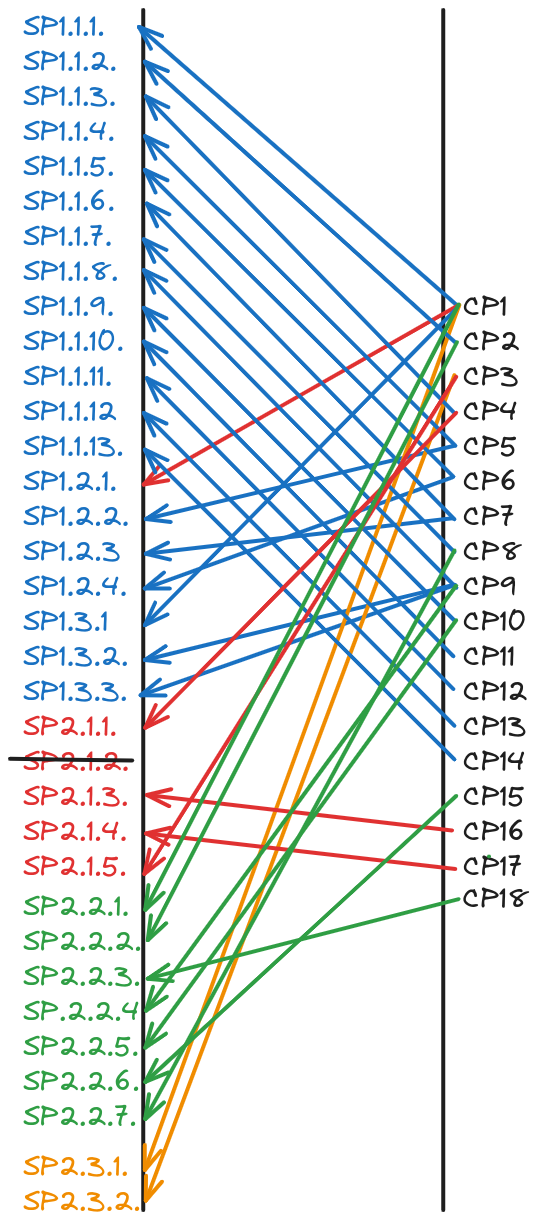
\includegraphics[width=\textwidth]{trazabilidad.png}
	\captionof{figure}{Trazabilidad del sistema}
\end{minipage}
